% ===========================================================================
\section{A contagem coerente}\label{sec:contagem}
% ===========================================================================

As seções anteriores desenham o crivo. Esta descreve um caso em que a
representação espectral deixa de ser um desenho e passa a ser um instrumento de
\emph{medição}, com uma propriedade que a aritmética não tem de graça: a altura de
um pico é uma contagem exata.

\subsection{Núcleos e órbitas}

Fixe um conjunto finito $P$ de primos, que chamaremos de \emph{base de remoção}.
Para $m\in\N$, o \emph{núcleo} de $m$ em relação a $P$ é a parte que sobra quando
se removem todos os fatores de $P$:
\[
  \nuc_P(m) \;=\; \frac{m}{\prod_{p\in P}p^{\,v_p(m)}} .
\]
A \emph{órbita} de um inteiro $P$-livre $r$ é
\[
  \mathcal{O}_r \;=\; \bigl\{\,m\in\N : \nuc_P(m)=r\,\bigr\}
  \;=\; \Bigl\{\,r\prod_{p\in P}p^{a_p} \in \N \,\Bigr\}_{a_p\ge0} .
\]
A órbita é a classe de equivalência de $m$ pela relação ``tem a mesma parte livre
de $P$''. Todos os seus elementos têm, por construção, o mesmo núcleo.

\begin{observacao}\label{obs:orbita}
A órbita $\mathcal O_r$ é o conjunto dos elementos de $\Lat(P)$ transladados de
$\nfreq r$. Em particular, se $r$ é um primo que não está em $P$, então $\nfreq r$
não pertence a $\Lat(P)$: o núcleo de $r$ é ele mesmo, e a órbita de $r$ é o
próprio $r$.
\end{observacao}

\subsection{A identidade de contagem}

Seja $\varphi\colon\N\to(0,\infty)$ uma função de peso, e considere o sinal
formado pela soma dos tons de todos os elementos de um lote $\mathcal L$, cada um
emitido na frequência do seu \emph{núcleo}:
\begin{equation}\label{eq:colapsado}
  R_{\mathcal L}(t) \;=\;
  \sum_{\substack{m\in\mathcal L\\ \nuc_P(m)>1}}
  \varphi\bigl(\nuc_P(m)\bigr)\,\cos\bigl(t\,\nfreq{\nuc_P(m)}\bigr) .
\end{equation}

\begin{proposicao}[contagem coerente]\label{prop:ganho}
Para cada $P$-livre $r>1$, seja $k_r=\#\{m\in\mathcal L:\nuc_P(m)=r\}$. Então a
componente de $R_{\mathcal L}$ na frequência $\nfreq r$ é exatamente
\[
  k_r\,\varphi(r)\,\cos\bigl(t\,\nfreq r\bigr).
\]
Em consequência, a razão entre o coeficiente de Fourier de $R_{\mathcal L}$ em
$\freq r$ e o coeficiente do sinal de um único termo de núcleo $r$ é exatamente
$k_r$ — para qualquer janela $T$, qualquer passo de amostragem e qualquer peso
$\varphi$.
\end{proposicao}

\begin{proof}
Por definição de núcleo, todos os $m\in\mathcal L$ com $\nuc_P(m)=r$ contribuem
em \eqref{eq:colapsado} com a \emph{mesma} função de $t$,
$\varphi(r)\cos(t\nfreq r)$. Somando $k_r$ cópias idênticas obtém-se
$k_r\varphi(r)\cos(t\nfreq r)$. A linearidade da transformada de Fourier preserva
a proporção, e o fator comum $\varphi(r)$ cancela na razão.
\end{proof}

A Proposição~\ref{prop:ganho} não tem conteúdo analítico: é a distributividade da
soma aplicada a termos idênticos. O que ela tem é uma consequência de leitura. Em
um espectro comum, a altura de um pico depende do tamanho do inteiro que o emite
(no nosso caso, $m^{-1/2}$ em \eqref{eq:serie}); dois inteiros diferentes nunca dão
a mesma altura, e comparar alturas exige calibrar. Aqui, todos os termos que caem
na mesma frequência são o mesmo termo, de modo que a altura relativa passa a medir
\emph{quantos} são. O espectro vira um contador.

\subsection{O detector de núcleo comum}

A leitura prática é imediata. Dado um lote de candidatos, forme o sinal
\eqref{eq:colapsado} e meça, para cada primo candidato a núcleo $r$, a razão
\[
  \widehat{k}_r \;=\;
  \frac{\text{amplitude medida em } \freq r}
       {\text{amplitude medida para um único termo de núcleo } r} .
\]
Pela Proposição~\ref{prop:ganho}, $\widehat k_r=k_r$ a menos do erro de medição, e
$k_r\ge2$ significa que $k_r$ candidatos do lote compartilham o núcleo $r$. Um
único espectro responde, simultaneamente, quais núcleos aparecem e quantas vezes.

A Figura~\ref{fig:contagem} mostra as duas verificações. À esquerda, o crescimento
com o número de termos: para $k=1,\dots,7$ candidatos com núcleo comum $11$, a
razão medida é $k$ com cinco casas decimais exatas — o erro é de arredondamento,
não de modelo. À direita, o caso cego: dezesseis inteiros, dos quais sete
compartilham o núcleo $11$, cinco o núcleo $13$ e quatro têm núcleos distintos. As
razões medidas são $6{,}99$ e $4{,}99$ nos dois núcleos compartilhados e ficam em
$1{,}00\pm0{,}01$ em todos os demais.

\begin{figure}[htbp]
\centering
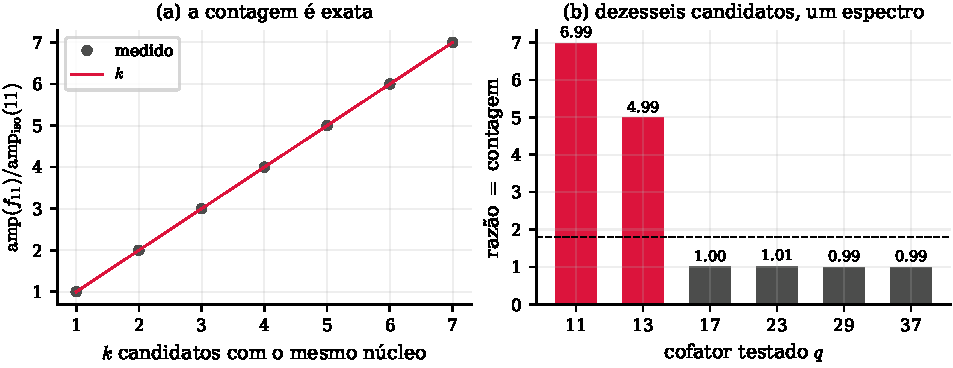
\includegraphics[width=0.95\textwidth]{figuras/f5_contagem.pdf}
\caption{(a) A razão medida em $\freq{11}$ para $k$ candidatos de núcleo comum,
com $k=1,\dots,7$; a reta é $\widehat k_{11}=k$. (b) Detecção em lote: dezesseis
candidatos, base $P=\{2,3,5,7\}$, um único espectro. As barras vermelhas são os
núcleos compartilhados, com altura igual à contagem.}
\label{fig:contagem}
\end{figure}

\begin{table}[htbp]
\centering
\small
\begin{tabular}{rrrr}
\toprule
núcleo $r$ & candidatos no lote & $\widehat k_r$ medido & erro \\
\midrule
$11$ & $7$ & $6{,}9897$ & $1{,}5\times10^{-3}$ \\
$13$ & $5$ & $4{,}9860$ & $2{,}8\times10^{-3}$ \\
$17$ & $1$ & $1{,}0010$ & $1{,}0\times10^{-3}$ \\
$23$ & $1$ & $1{,}0052$ & $5{,}2\times10^{-3}$ \\
$29$ & $1$ & $0{,}9932$ & $6{,}8\times10^{-3}$ \\
$37$ & $1$ & $0{,}9911$ & $8{,}9\times10^{-3}$ \\
\bottomrule
\end{tabular}
\caption{Leitura de um único espectro para dezesseis candidatos
($T=6500$, $\Delta t=5\times10^{-4}$). Os núcleos não compartilhados ficam em
torno de $1$, dentro do erro de lotação espectral.}
\label{tab:contagem}
\end{table}

\subsection{Três observações honestas}

\paragraph{A construção usa aritmética.} Para escrever \eqref{eq:colapsado} é
preciso calcular $v_p(m)$ de cada candidato, isto é, dividir. O que é espectral é a
\emph{medição}, não a preparação. A representação da Seção~\ref{sec:dicionario} é
fiel, mas não é gratuita: o núcleo é um dado aritmético antes de ser uma
frequência.

\paragraph{O que se mede é multiplicidade, não primalidade.} O detector conta
quantos candidatos compartilham um núcleo; ele não decide se o núcleo é primo nem
se os candidatos são. Se o núcleo for composto, o pico aparece em $\freq r$ com
$r$ composto, e a contagem continua correta. A proposição é sobre somas de termos
idênticos, não sobre aritmética dos termos.

\paragraph{O custo é o da janela.} Pela Proposição~\ref{prop:janela}, os núcleos
precisam estar resolvidos uns dos outros: se dois núcleos têm frequências muito
próximas, a faixa de leitura de um invade o outro e as contagens se contaminam. O
comprimento de janela necessário é $\tau$-como na Seção~\ref{sec:resolucao} — da
ordem do maior núcleo presente. Para lotes pequenos e núcleos pequenos, isso é
barato; para núcleos grandes, não é.

\subsection{Uma variante: potências}

A identidade não depende de os núcleos serem primos. Se um inteiro $m$ tem núcleo
$r=11^2$, o termo aparece em $\freq{121}$; se depois se remove um fator $11$, ele
migra para $\freq{11}$ e passa a somar com os demais. A contagem pode assim ser
feita em camadas: primeiro o núcleo completo, depois os núcleos sucessivos obtidos
removendo um fator de cada vez. Cada camada é um novo sinal
\eqref{eq:colapsado} e uma nova contagem exata.

Essa observação é o análogo, no dicionário, do que a fatoração por divisões
sucessivas faz na aritmética: ela desce a árvore de fatores por níveis. A
diferença é de leitura — na aritmética, o resultado é o quociente; aqui, é a
posição do pico no nível seguinte.
